\section{Hallwachs-Experiment} \label{sec:hallwachs}
Mit dem Hallwachs Experiment entdeckte Wilhelm Hallwachs 1888 den fotoelektischen Effekt, der die klassische (mechanische) Wellentheorie widerlegte und das Kapitel der Quantenphysik öffnete.

\subsection{Aufbau und Beobachtung}

Die geladene Zinkplatte eines Ladungsmesser (Siehe: \referenz{subsec:Elektroskop}) wird zunächst mit weißem Licht bestrahlt, wobei sich keine Veränderung des Ausschlags der Nadel zeigt. Auch beim Hinzunehmen weiter identischer Lichtquellen, also einer Erhöhung der Intensität des Lichts, gibt es keine Veränderung.

Beim Wiederholung des Versuches mit Ultraviolettlicht, welches ein kürzere Wellenlänge besitzt, wird allerdings der Ausschlag der Nadel kleiner.

\subsection{Deutung nach Hallwachs}

Elektronen wurden aus der Metallplatte gelöst, daher kommt die Veränderung des Nadelausschlags. Daraus folgt, dass die Energie von elektromagnetischer Wellen abhängig von der Wellenlänge ist und \textbf{nicht} von der Intensität. \textbf{Dies ist ein Widerspruch zur klassischen Wellentheorie.}

Licht muss also neben dem Wellencharakter (Siehe: \kapitelreferenz{ch:Optik}) auch Teilchencharakter zeigen. Dieses Lichtteilchen nennt man \glqq Photon\grqq .

\section{Fotoeffekt} \label{sec:fotoeffekt}
Der Fotoeffekt ist der heutige Name für den Hallwachseffekt und die Erforschung und Mathematisierung erfolgte von Max Planck und Albert Einstein Anfang des 20. Jahrhunderts.

Nun war qualitativ bekannt, dass Licht ab einer bestimmten Wellenlänge Elektronen aus Metall auslöst, allerdings gab es weder eine quantitative Bestimmung der Menge dieser Elektronen, noch eine Gleichung zur Bestimmung der Strahlungsenergie.

\begin{NiceToKnow}
	Qualitative Bestimmung heißt, man kann das Ergebnis eines Versuches so vorhersagen, dass man zwar den Effekt kennt und Aussagen über Dinge wie Richtung einer möglichen Bewegung, etc. machen kann, aber keine exakten Werte angeben kann.
	
	Mit einer quantitativen Aussage gibt man auch exakte Werte an.
\end{NiceToKnow}


\subsection{Fotozelle}

Bei dem Experiment kommt die sogenannte Fotozelle zum Einsatz.

Eine Fotozelle ist ein evakuierter (im Inneren ist ein Vakuum) Glaszylinder, in welchem sich, im gröbsten Sinne, ein Kondensator befindet. An zwei Elektroden die sich im Inneren befinden, eine ist ringförmig und die andere halbkugelförmig, lassen sich Messgeräte und Spannungsquellen anschließen.
%Cue for pic

\subsection{Aufbau und Durchführung}

Eine Fotozelle wird mit UV-Licht bestrahlt, dadurch werden Elektronen Elektronen aus der schalenförmigen Kathode aus Natrium (ein Metall) ausgelöst. 

Es kann beobachtet werden, dass ein (wenn auch extrem kleiner) Strom fließt, wenn man die beiden Elektronen über einen Widerstand und ein Strommessgerät verbindet.

Eine Gegenspannung $U_{max}$ wird an der Fotozelle angelegt und so lange erhöht, bis kein Strom $I$ mehr gemessen wird.


\subsection{Deutung}

Einige der herausgeschlagenen Elektronen treffen auf der ringförmigen Anode auf; dies erzeugt den Strom der gemessen wird.

Diese Elektronen besitzen eine demnach eine kinetische Energie $E_{kin}$ (Siehe: \referenz{subsec:Energieformen}), wenn sie ausgelöst werden. Durch die Gegenspannung müssen sie gegen ein entgegengesetztes elektrisches Feld "ankämpfen" (Siehe: \referenz{sec:ElektronenwegungImEFeld}). Wenn kein Strom $I$ mehr gemessen wird ist die elektrische Energie $E_{el} = U \cdot e$ (Siehe: \gleichungsreferenz{eq:arbeit_kondensator} mit der Feldstärke $E$ (nicht verwechseln mit der Energie, beides hat das Formelzeichen $E$) im Kondensator $E=\frac{U}{d}$) gleich der kinetischen Energie $E_{kin} = \frac{1}{2} m v^2$ (Siehe: \gleichungsreferenz{eq:ekin}):

\begin{align}
\begin{split}
	E_{el} &= E_{kin} \\
\end{split}
\end{align}


\subsection{Photonenenergie}

Nun kann man davon ausgehen, dass die Energie \emph{eines} Lichtphotons gleich der kinetischen Energie \emph{eines} ausgelösten Elektrons ist. Da es, durch andere Faktoren, Unterschiede in den Geschwindigkeiten der herausgeschlagenen Elektronen gibt, werden nur die schnellsten, also die energiereichsten Elektronen in Betracht gezogen. 

Es gibt allerdings eine gewisse Austrittsarbeit $W_A$, abhängig von dem Material der Kathode, die notwendig ist, um ein Elektron überhaupt aus der Platte zu lösen, ohne im dabei eine kinetische Energie mitzugeben. Daher muss diese Größe von der Photonenenergie $E_{phot}$ abgezogen werden.

Ferner ist $E_{kin}$, wie gerade gezeigt, gleich $E_{el}$, sodass man schreiben kann:

\begin{align} \label{eq:EelmitWA}
\begin{split}
	E_{el} &= E_{phot} - W_A \\
\end{split}
\end{align}

\begin{figure}[h!]
	\centering
	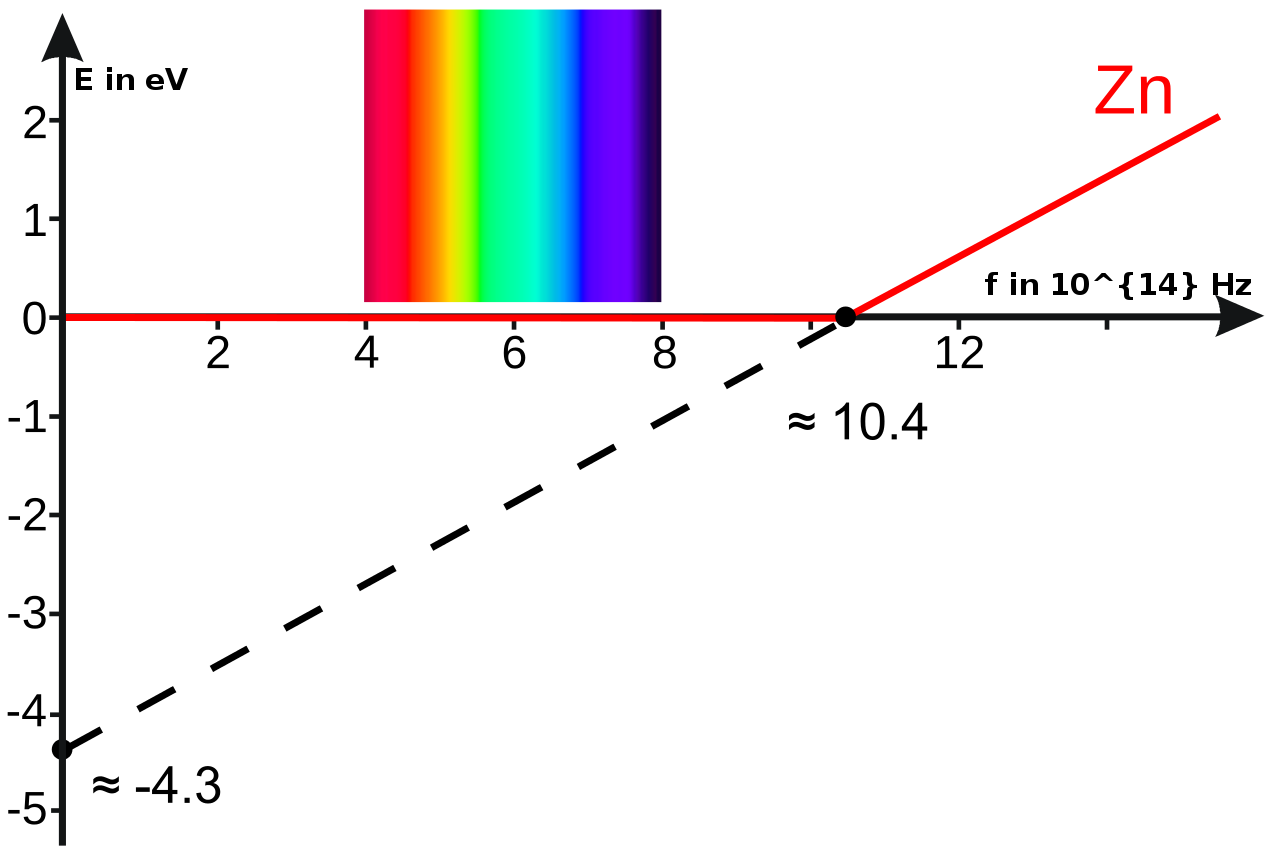
\includegraphics[width=0.7\textwidth]{PhotoelektischerEffekt}
	\caption{Aufführung der Energie der Elektronen (in Elektronenvolt: $1 eV = q_e J \approx 1,602 J$) über der Frequenz des Lichtes. Ein Spektrum gibt eine Referenz des Bereiches.}
	\label{fig:Fotoeffekt}
\end{figure}

Aus der Abbildung \ref{fig:Fotoeffekt}\endnote{\glqq Photoelectric effect diagram no label\grqq{} by Klaus-Dieter Keller - File:Photoelectric effect diagram.svg. Licensed under CC BY 3.0 via Wikimedia Commons. Modified by Till Blaha (Labeling) - \url{https://commons.wikimedia.org/wiki/File:Photoelectric_effect_diagram_no_label.svg}} ist ein linearer Anstieg der Photonenenergie ersichtlich. Max Planck folgerte daraus, dass es ein Naturkonstante gibt, die die Steigung definiert.

Einstein formulierte dann die, sehr wichtige, Einstein'sche Gleichung:

\begin{align}	\label{eq:einsteinscheGleichung}
\begin{split}
	E_{phot} = h \cdot f
\end{split}
\end{align}

\noindent Hierbei ist $h$ das \glqq Plank'sche Wirkungsquantum\grqq , eine Naturkonstante (\casio{06}), mit:

\begin{equation}
	h \approx 6,626 \cdot 10^{-34} Js = 6,626 \cdot 10^{-34} \frac{kg \cdot m^2}{s}
\end{equation}


\subsection{Austrittsarbeit}

Mit Gleichung \ref{eq:einsteinscheGleichung} kann man die Gleichung \ref{eq:EelmitWA} weiter auflösen und erhält für $W_A$:

\begin{align} \label{eq:Austrittsarbeit}
\begin{split}
	E_{el} &= h \cdot f - W_A \\
	e \cdot U &= h \cdot f - W_A \\
	W_A &= h \cdot f - e \cdot U
\end{split}
\end{align}


\subsection{Grenzfrequenz}

Für die Grenzfrequenz $f_{gr}$, also die Frequenz, die das Licht mindestens haben muss, um Elektronen aus einem bestimmten Material zu lösen, lässt sich aus Gleichung \ref{eq:EelmitWA} ableiten, wenn man $E{el} = 0$ setzt:

\begin{align} \label{eq:Grenzfrequenz}
\begin{split}
	0 &= E_{phot,gr} - W_A \\
	W_A &= E_{phot,gr} \\
	W_A &= h \cdot f_{gr} \\
	f_{gr} &= \frac{W_A}{h}
\end{split}
\end{align}




\section{Ist Licht ein Teilchen oder eine Welle?} \label{sec:lichtteilchenwelle}
\begin{itemize}
\item Licht als Welle:
	\begin{itemize}
	\item Bei Wellenoptik, Hygens'sches Prinzip, elektromagnetische Welle (E-Feld, B-Feld)
	\item Brechung, Reflexion, Polarisation
	\item Doppelspalt, Einzelspalt
	\end{itemize}
\item Licht als Teilchen:
	\begin{itemize}
	\item Immer wenn von Licht als Photon die Rede ist.
	\item Fotoeffekt, Compton-Streuung
	\item Photonenimpuls
	\end{itemize}
\end{itemize}

\section{Photonenimpuls} \label{sec:photonenimpuls}
\begin{itemize}
\item Der Impuls $\vec{p}$ eines beliebigen Körpers mit Masse ist definiert als: 

$\vec{p} = m \cdot \vec{v}$
\item Photonen haben aber keine Ruhemasse. Ihre Masse lässt sich nur durch Umformen der Gleichung der speziellen Relativitätstheorie $E = mc^2$ ermitteln.

$m = \frac{E}{c^2}$

daraus folgt:

$\vec{p} = \frac{E}{c^2} \cdot \vec{c}$ \tabto{0.5\textwidth} ; $\vec{v} = \vec{c}$ da Photonen sich stets mit Lichtgeschwindigkeit fortbewegen.

$\vec{p} = \frac{h \cdot f}{\vec{c}}$ \tabto{0.5\textwidth} ; $E_{phot} = h \cdot f$

$\vec{p} = \frac{h}{\lambda \cdot f}$ \tabto{0.5\textwidth} ; $c = \lambda \cdot f$

$\vec{p} = \frac{h}{\lambda}$
\item Das heißt das, dass alles mit einem Impuls eine Wellenlänge hat, \referenz{sec:debroglie}
\item Nice to know: $F = \frac{\Delta p}{\Delta t}$
\end{itemize}

\subsection{Elastischer Stoß}
\begin{itemize}
\item Bei einem elastischen Stoß bleibt die Summe der kinetischen Energien der Stoßpartner unverändert.

$\frac{1}{2}m_1 \cdot v_1^2 = \frac{1}{2}m_1 \cdot (v'_1)^2 + \frac{1}{2}m_2 \cdot (v'_2)^2$
\item Wenn $m_1 << m_2$ (wie bei Experiment Lichtmühle bzw. Photon Reflektor) ist $v'_1 \approx -v_1$ und $\vec{p'} \approx -2 \vec{p}$
\end{itemize}

\subsection{Unelastischer Stoß}
\begin{itemize}
\item Der Vorgang ist nicht reibungsfrei, es geht kinetische Energie "verloren" (Umwandlung in Wärme).
\item Beispiel Elektronen auf schwarze Fläche, es kommt nur zum einfachen Impulsübertrag, die verlorene Energie wird in Wärme umgewandelt.
\end{itemize}




\section{De Broglie Wellenlänge} \label{sec:debroglie}
Der Physiker Louis De Broglie erkannte aus der Impulsgleichung des Photons (\gleichungsreferenz{eq:Photonenimpuls}), dass mathematische gesehen, jedes Teilchen mit einem Impuls, also jedes Teilchen, bzw. jeder Körper, mit einer Masse und einer Geschwindigkeit, eine Wellenlänge hat.

Diese Art der Welle nennt man auch Materialwelle oder De-Broglie-Welle.

Die Berechnung der De-Broglie-Wellenlänge gestaltet sich denkbar einfach. Aus Gleichung \ref{eq:Photonenimpuls} geht hervor:

\begin{equation}
	\lambda_{dB} = \frac{h}{p} = \frac{h}{m \cdot v}
\end{equation}

\section{Interferenzen von Quantenobjekten} \label{sec:interferenzenquanten}
\begin{itemize}
\item Aufgrund der De Broglie-Wellenlänge haben Elektronen eine Wellenlänge, wenn sie einen Impuls besitzen.
\item Die Wellenlänge eines Elektron ist bei bestimmten Konfigurationen groß genug, dass Interferenzerscheinungen auftreten (Das Elektron \textbf{verhält} sich wie eine Welle, ist aber keine.)
\item Theoretisch lässt sich seinen Wellenlänge $\lambda$ durch das Gleichsetzen der Gleichung des Impulses $\vec{p}=m\cdot\vec{v}$ mit der Formel für den Photonenimpuls $\vec{p}=\frac{h}{\lambda}$:

$m\cdot\vec{v}=\frac{h}{\lambda}$ \tabto{0.5\textwidth} ; umstellen nach $\lambda$

$\lambda = \frac{h}{m \cdot v} $

\item Um die Geschwindigkeit $v$, bei einem Versuch mit Elektronenbeschleunigung durch ein elektrisches Feld, zu ersetzen, setzt man zunächst die Gleichungen der kinetischen Energie $E_{kin}$ mit der Gleichung der Elektrischen $E_{el}$ gleich und formt anschließend nach $v$ um.

$\frac{1}{2} m_e \cdot v^2 = e \cdot U_a$ \tabto{0.5\textwidth} ; $U_a$ ist die Beschleunigungsspannung, mit der das Elektron in dem jeweiligen Versuch beschleunigt wurde.

$v = \sqrt{\frac{2e \cdot U_a}{m_e}}$

durch Einsetzen folgt dann:

\Large $\lambda = \frac{h \sqrt{m_e}}{m \cdot \sqrt{2e \cdot U_a}} $
\end{itemize}

\subsection{...an Grafit}
\begin{itemize}
\item Da Elektronen demnach eine sehr kleine Wellenlänge haben, benutzt man oft Kristalle um Interferenzmuster zu erzeugen.
\item An den Netzebenen des Kristalls, in denen die Atome regelmäßig angeordnet sind, werden Elektronen, ähnlich wie Licht an dünnen Schichten (Glimmer), gestreut.
\item Auf dem Leuchtschirm der Röhre kommt es je nach Gangunterschied über die verschiedenen Netzebenen zu Maxima und Minima.
\item Wichtig: Bei Grafit haben die Atome in einer Ebene einen anderen Abstand d zu einander, als die Atome zwischen den Ebenen. Es gibt als zwei "Spaltabstände" und folglich auch zwei Maxima 1. (2.,...,n.) Ordnung.

\item Der Gangunterschied $\delta = 2d\cdot\sin{\alpha} $ für konstruktive Interferenz muss ein natürliches vielfaches der Wellenlänge $\lambda$ sein.

$n \cdot \lambda = 2d \cdot \sin{\alpha}$

\Large $\sin{\alpha} = \frac{n \cdot \lambda}{2d}$ Bragg'sche Bedingung / Gleichung
\end{itemize}

Achtung in der Zeichnung ist $\alpha$ mit $\Theta$ vertauscht!

\begin{figure}[h!]
\centering 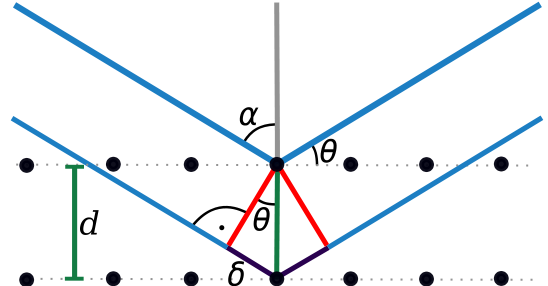
\includegraphics[width=0.8\textwidth]{Streuung_an_Graphit}
\caption{Abbildung von: \url{https://upload.wikimedia.org/wikipedia/commons/thumb/c/ca/Bragg.svg/548px-Bragg.svg.png}}
\end{figure}



\subsubsection{Versuch}
\begin{itemize}
\item Im Versuch wird ein Elektronenstrahl auf einen Graphitkristall geleitet, an diesem kommt es zu Streuung und es bilden sich jeweils zwei ringförmige Maxima auf dem Schirm.
\item Bezeichnet man den Abstand vom Maximum n. Ordnung zum Maximum 0. Ordnung mit $r$ und den Abstand vom Kristall zum Schirm mit $l$ folgt:

$\tan{2\alpha} = \frac{r}{l}$
\item Um die Wellenlänge der Elektronen experimentell zu bestimmen, setzten wir dies Formel mit der Bragg'schen Gleichung gleich.

$2\sin{\alpha} = tan{2\alpha}$

wendet man die Kleinwinkelnäherung an, folgt: \\
\Large $\frac{n\cdot\lambda}{2d}=\frac{r}{l}$

\normalsize

umgestellt nach $\lambda$:\\
\Large $\lambda = \frac{2dr}{n\cdot l}$

\normalsize

ohne Winkelnäherung:\\
\Large $2\cdot\arcsin(\frac{n\cdot \lambda}{2d})=\arctan(\frac{r}{l}) $

\Large $\arcsin(\frac{n\cdot \lambda}{2d})=\frac{1}{2}\cdot\arctan(\frac{r}{l})$ 

\Large $\frac{n\cdot \lambda}{2d}=\sin(\frac{1}{2}\cdot\arctan(\frac{r}{l}))$ 

\Large $\lambda=\sin(\frac{1}{2}\cdot\arctan(\frac{r}{l}))\cdot 2d \cdot \frac{1}{n}$ \tabto{0.5\textwidth} ; meistens ist n=1 

\normalsize

\item Nice to know: Es kommt nur zur Interferenz, wenn die Bragg'sche Gleichung erfüllt ist. Dafür muss $\alpha$, für eine bestimmte Wellenlänge, auch eine bestimmte Größe haben. Im Experiment wird deshalb eine Graphitfolie benutzt, auf der die Kristallgitter in den verschiedensten Anordnungen liegen. So ist statistisch gesehen immer ein Kristall im richtigen Winkel zum Elektronenstrahl.
\end{itemize}

\subsection{...am Doppelstpalt}
\begin{itemize}
\item Grundsätzlich gelten die gleichen Formeln wie bei Interferenz mit Licht. Allerdings muss der Spaltabstand $d$, aufgrund der ebenfalls sehr kleinen Wellenlängen, sehr klein sein, um überhaupt ein Interferenzmuster detektieren zu kommen.\\
Das Interferenz Muster ist so klein, dass man es nur mit einem Elektronenmikroskop sichtbar machen kann.
\item Bedingungen für konstruktive Interferenz: $\delta = n \cdot \lambda$\\
für destruktive Interferenz: $\delta = (n-\frac{1}{2}) \cdot \lambda$
\end{itemize}

\subsubsection{Versuch}
\begin{itemize}
\item Um die Wellenlänge $\lambda$ experimentell herauszufinden, gilt, wenn $d$ der Spaltabstand ist, $a$ der Abstand zum Schirm und $d_k$ der Abstand des k. Maximum zum 0. Maximum ist:

$\tan{\alpha}=\frac{d_k}{a}$ und $\sin{\alpha}=\frac{k \cdot\lambda}{d}$

Dann entweder durch Kleinwinkelnäherung:\\
\Large $\lambda = \frac{d_k \cdot d}{k \cdot a}$

\normalsize oder ohne:

\Large $\lambda = \sin(\arctan(\frac{d_k}{a})) \cdot \frac{d}{k}$
\end{itemize}

\section{Compton Wellenlänge} \label{sec:compton}
Wenn man Photonen mit ausreichend Energie (ab ca. 100keV) auf gebundene Elektronen schießt, wird das Phänomen durch den Fotoeffekt (Siehe \referenz{sec:fotoeffekt}) beschrieben. Es kommt zur vollständigen Impulsübertragung vom Photon auf das Elektron.

Wenn man ein Photon nun gegen ein freies Elektron schießt, wird das Phänomen durch den Compton-Effekt beschrieben:

\subsection{Effekt}

Es kommt nicht immer zu einer vollständigen Impulsübertrag, nämlich kann das Elektron auch zur Seite abgelenkt und das Photon dann in der Konsequenz nicht in die entgegengesetzte Richtung reflektiert. Wenn nicht der ganze Impuls übertragen wird, kommt es zur Compton-Streuung. 

Das Elektron wird in eine Richtung wird durch den Teilimpuls in eine Richtung beschleunigt, und das Photon wird in eine andere abgelenkt. Nach dem Zusammenstoß hat das Photon einen geringeren Impuls, und da seine Geschwindigkeit konstant $c$ ist, ändert sich, bedingt durch den Impulserhaltungssatz, seine Wellenlänge (sie wird größer).

\begin{comment}\item Durch den Impulserhaltungssatz gilt:\\
Vor Kollision:\\
$p_{gesamt} = p_{Phot} \rightarrow p_{gesamt}=\frac{h}{\lambda}$


Nach Kollision: \\
$p_{gesamt} = p'_{phot} + p_e$

$\frac{h}{\lambda} = \frac{h}{\lambda'} + m_e \cdot v$

$\frac{h}{\lambda} = \frac{h}{\lambda} \cdot \cos{\Theta} + \frac{h}{\lambda} \cdot (1-\cos{\Theta})$ \tabto{0.5\textwidth} ; $c = \lambda * f \rightarrow \lambda = c / f$

$\frac{h}{\lambda} = \frac{h}{\lambda} \cdot \cos{\Theta} + \frac{h}{\lambda} \cdot (1-\cos{\Theta})$





$m_e \cdot v = \frac{h}{\lambda}$ \tabto{0.5\textwidth} ; umstellen nach $\lambda$ 


$\lambda' = \lambda + \Delta\lambda$

$\lambda' - \lambda = \Delta\lambda$

$\lambda' - \lambda = $


$\lambda = \frac{h}{m_e \cdot v}$

\end{comment}

\begin{comment}
Vor Kollision:\\
$p_{gesamt} = p_{phot}$

Nach Kollision: \\
$p_{gesamt} = p'_{phot} + p_{Teilchen, an dem gestreut}$

Für $\Delta p$: \\
$p_{gesamt} - p'_{phot} = \Delta p$ \tabto{0.5\textwidth} ; umstellen nach $p_{gesamt}$ \\
$p_{gesamt} = \Delta p + p'_{phot}$ \\

Einsetzen in die Gesamtgleichung für nach Kollision:\\
$\frac{h}{\Delta \lambda} + \frac{h}{\lambda '} = \frac{h}{\lambda '} + m \cdot v$ \tabto{0.5\textwidth} ; mit $p_{Teilchen, an dem gestreut} = m \cdot v$ \\
$\frac{h}{\Delta \lambda} = m \cdot v$ \\
$\frac{h}{\Delta \lambda \cdot m \cdot v} = 1$ \\
$\Delta \lambda = \lambda_c = \frac{h}{m \cdot v}$ \\


\end{comment}

\begin{comment}
\item Compton-Wellenlänge hergeleitet:

Durch den Impulserhaltungssatz gilt:\\

Vor Kollision:\\
$p_{gesamt} = p_{phot}$

Nach Kollision: \\
$p_{gesamt} = p'_{phot} + p_{Teilchen, \ an \ dem \ gestreut}$

Für $\Delta p$: \\
$\Delta p = p_{phot} - p'_{phot}$

$\Delta p = p_{gesamt} - p'_{phot}$ \tabto{0.5\textwidth} ; umstellen nach $p_{gesamt}$

$p_{gesamt} = \Delta p + p'_{phot}$ \\


Einsetzen in die Gesamtgleichung für "nach Kollision": \\
$\frac{h}{\Delta \lambda} + \frac{h}{\lambda '} = \frac{h}{\lambda '} + m \cdot v$ \tabto{0.5\textwidth} ; mit $p_{Teilchen, \ an \ dem \ gestreut} = m \cdot v$

$\frac{h}{\Delta \lambda} = m \cdot v$ \\

Dann noch nach $\Delta \lambda$ umformen und man erhält die Compton Wellenlänge: \\
$\Delta \lambda = \lambda_c = \frac{h}{m \cdot v}$ \\
\end{comment}

Für ein Elektron als Teilchen, an dem gestreut wird, gilt die Compton-Wellenlänge des Elektrons (\casio{12}):

\begin{equation}
	\Delta \lambda = \lambda_c = \frac{h}{m_e \cdot v} \approx 2,426 \cdot 10^{-12}m
\end{equation}

Wenn $\lambda$ die Wellenlänge des Lichts vor dem Stoß und $\lambda'$ die Wellenlänge nach dem Stoß, dann ist die Wellenlängenänderung, in Abhängigkeit des Streuungswinkels $\Theta$:

\begin{align}
\begin{split}
	\lambda' - \lambda &= \frac{h}{m \cdot c}-\frac{h}{m \cdot c} \cos{\Theta} \\
	\Delta\lambda &= \frac{h}{m \cdot c}(1-\cos{\Theta}) \\
	\Delta\lambda &= \lambda_c \cdot (1-\cos{\Theta})
\end{split}
\end{align}


\noindent Das Maximum dieser Gleichung liegt bei $\Theta = 180\degree \rightarrow (1-\cos{180\degree})=2$. \\
Das Minimum ist bei $\Theta = 0\degree \rightarrow (1-\cos{0\degree})=0$.


\section{Beschreibung von Quantenobjekten} \label{sec:beschreibungquanten}
Als man den Versuch mit Elektronen am Doppelspalt durchführte, tat man dies auch mit einzelnen Elektronen, die nacheinander auf den Spalt \glqq abgefeuert\grqq{} wurden und stellte fest, dass auch bei dieser Konfiguration das Interferenzmuster auftrat.

Um den Versuch noch genauer zu untersuchen und zu überwachen, brachte man einen Detektor an einem der Spalte an, um festzustellen, durch welchen Spalt sich das Elektron bewegt. Als man dies aber tat, traten keine Interferenzen mehr auf, was man am Bild der Elektronen auf dem Schirm erkennen konnte.

Diese Entdeckung ließ und lässt sehr viele Fragen auf, aber stellte klar, dass man das Verhalten von Quantenobjekte nicht vorhersagen und nicht einmal vollständig beschreiben kann, sondern Aussagen nur mit Wahrscheinlichkeiten treffen kann.

\section{Heisenbergsche Unbestimmtheitsrelation} \label{sec:unbestimmtheitsrelation}
Werner Heisenberg fand heraus, dass man bei Quantenobjekten, z.B. Elektronen, nie den Aufenthaltsort \emph{und} den Impuls, also die Geschwindigkeit und die Richtung (Im Impulse steckt die Geschwindigkeit, eine gerichtete Größe), genau bestimmen kann. Das hat nichts mit den Ungenauigkeiten von Messtechniken zu tun, sondern ist ein Phänomen.

Er stellte die Heisenbergsche Unbestimmtheitsrelation auf, auch Unschärferelation genannt:

\begin{align}
\begin{split}
	\Delta x \cdot \Delta p \ge \frac{h}{4\pi}
\end{split}
\end{align}

Hierbei ist $\Delta x$ die Ortsunschärfe und $\Delta p$ die Impulsunschärfe. Dies sind die Genauigkeitsbereiche, mit denen die beiden Größen bestimmt werden können. Wenn man also nun den Ort genau bestimmen kann, kann man den Impuls nur ungenau bestimmen und daher nicht genau vorhersagen, wie schnell oder in welche Richtung sich das Teilchen fortbewegen wird.

Auf Elektronen am Doppelspalt angewendet bedeutet das, dass man, auch wenn der Ort des Elektrons sehr genau bestimmt werden kann (es kann sich ja nur durch einen der beiden Spalte bewegen und dort kann man Detektoren anbringen), nicht sicher weiß, wohin es sich bewegt, da man zwar weiß, aus welcher Richtung es kam, aber die Ablenkung am Doppelspalt und daher den Impuls und die weitere Flugbahn, nicht genau bestimmen kann.

